\section{Implementation}
傳統的 Q Learning 會使用一個 Q table 來記錄每個 state - action pair 的預期回報,但這會遇到一個問題,就是狀態空間過大,如果再乘上可以選擇的 action 數量,這個 table 可能會大到根本無法建立。

所以 DQN 的設計是使用一個神經網路來估計 Q value,這樣一來就可以避免狀態空間過大的問題。

\subsection{How do you modify DQN to Double DQN?}
原始的 DQN 會遇到一個問題就是 Q value 高估的問題,這是因為在 Q 值得估計中,會有模型的 noise 混入,如果每次都選擇最大的 Q value 會有遇到每次都選擇 noise 的最大值,這並不能幫助我們學習,所以 Double DQN 的設計是使用兩個 Q network ,一個來選擇 action,另一個來估計 Q value ,這樣即使我們在選擇 action 的時候選擇了 因為 noise 的存在,而被高估的動作,但是由於計算最終的 Q value 時,我們會使用另一個 Q network 來計算,所以我們有理由相信,同時被高估的機率很小。

考慮到 DQN 的 Loss 設計是希望,當前預計的未來 Reward,與先採取一步驟再估計未來這一步驟採取之後的 Reward 要一致,所以我們把估計下一步的 Q value 使用一個 target network 來估計,這樣一來,就可以透過一直對未來的估計,來專注在提高當前選擇的 Reward。

目標是讓這左右兩式一致:
$$
r + \gamma \max_{a'} Q(s', a'; \bar{\theta}) \approx Q(s, a; \theta)
$$
如果過於頻繁的更新 network 的參數,會有 Online network 沒辦法好好收斂,建立策略。

\subsection{How do you obtain the Bellman error for DQN?}
下一個問題就是,在每次更新的時候,我們可以直接使用過去的 N 次狀態轉移來更新網路,也可以從記憶的資料庫中,隨機抽取 N 次狀態轉移來更新網路,但是直觀上,我們能夠理解有些記憶會特別有價值,如果是很常見的記憶,則沒有辦法帶給模型更多的知識。

所以 PER 的設計是,我們會使用一個優先權來衡量每個記憶的價值,這樣一來,我們就可以更關注在那些更少見,但是更有價值的記憶上。 那們如何衡量記憶的價值呢? 就是透過「令人驚訝」的程度來代表「有訊息量」,然後就優先抽取這些令人驚訝的數據進行學習,這裡就導入 TD error 的概念,因為 TD error 越大的話,就代表我們對於未來的估計越不準確,所以這些數據就更有價值。

這裡使用當前的估計,叫做current estimate,與多做一步之後的估計,叫做target estimate,這兩個估計的差值,就是 TD error (Temporal Difference error)。

$$
\delta = [r + \gamma \max_{a'} Q(s', a'; \bar{\theta})] - [Q(s, a; \theta)]
$$

Bellman error 是 TD error 的絕對值,所以可以寫成:

$$
p_i = \left| \delta_i \right| + \epsilon
$$

使用這個 Bellman error 來衡量記憶的價值,我們就可以更關注在那些更少見,但是更有價值的記憶上。


\subsection{How do you implement the memory buffer for PER?}

透過 np 提供的抽樣函數,我們可以給定不同的機率數值,來達到關注那些更少見、更令人驚訝的記憶。
透過 Bellman error 我們可以衡量記憶的價值,接下來就要把這個價值傳遞給抽樣函數,這時候會有 $\alpha$ 來退火,調整機率的敏感度,之後在用 $\beta$ 來平衡探索與利用。

\begin{lstlisting}[language=Python, caption=使用 np.random.choice 來抽樣記憶。]
indices = np.random.choice(len(self.buffer), batch_size, p=probs, replace=True)
\end{lstlisting}

\subsection{How do you modify the 1-step return to multi-step return?}
考慮 TD error 是代表,當前的估計 Reward 與多做一步之後的估計 Reward 的差值,所以如果我們多確定一些步驟,然後在計算 TD error 的時候,可以讓 loss 更準確的指導 model 更新的方向。 這也就是 multi-step return 的概念。

以 4 step 為例,我們可以在現在時間估計未來的 Reward ,然後過 4 個 sample 之後,有了 4 個真實的 Reward 之後,這時候我們就可以計算真實的 Reward 加對未來的估計,之後跟 4 個 sample 之前的估計做比較與指導模型更新。

\subsection{Explain how you use Weight \& Bias to track the model performance.}
由於這個專案的訓練過程中,我們會需要嘗試各種各樣的參數,所以會使用 Weight and Bias 來管理多台電腦的數據,尤其是比較不同數的曲線變化時特別好用。

\begin{figure}[htbp]
    \centering
    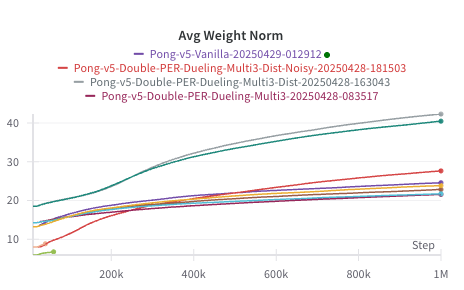
\includegraphics[width=0.8\textwidth]{figures/Avg_Weight_Norm.png}
    \caption{訓練過程中權重範數的平均值變化。}
    \label{fig:weight_norm}
\end{figure}

一開始由於 Reward 一直趴在 -21,所以我很擔心模型的 loss 並沒有傳遞進去模型中,去優化模型,所以我繪製了 Avg\_Weight\_Norm 的曲線,可以看到在訓練過程中,權重有持續變大,讓我確認到沒有 Loss 傳遞的 bug,令我意外的是,我可以透過比較 Avg\_Weight\_Norm 的曲線,來比較不同模型的訓練效果,這對於我們這種需要嘗試很多不同參數的狀況下,是非常有幫助的。

在開頭提到的 NoisyLayer 的設計,可以從這個圖觀察到他的 模型有更快的成長速度,雖然這並不代表 Reward 指標,但透過 Weight \& Bias 的協助,我們可以很快的得到這種需要比較的理解。
